% !TeX spellcheck = en_GB
%%%%%%%%%%%%%%%%%%%%%%%%%%%%%%%%%%%%%%%%%%
%                                        %
%    Engineer thesis LaTeX template      % 
%                                        %
%%%%%%%%%%%%%%%%%%%%%%%%%%%%%%%%%%%%%%%%%%



\documentclass[a4paper,twoside,12pt]{book}
\usepackage[utf8]{inputenc}                                      
\usepackage[T1]{fontenc}  
\usepackage{amsmath,amsfonts,amssymb,amsthm}
\usepackage[polish,british]{babel} 
\usepackage{indentfirst}
\usepackage{lmodern}
\usepackage{graphicx} 
\usepackage{hyperref}
\usepackage{booktabs}
\usepackage{tikz}
\usepackage{pgfplots}
\usepackage{mathtools}
\usepackage{geometry}
\usepackage[page]{appendix} 

\usepackage{setspace}
\onehalfspacing


\frenchspacing

\usepackage{listings}
\lstset{
	language={},
	basicstyle=\ttfamily,
	keywordstyle=\lst@ifdisplaystyle\color{blue}\fi,
	commentstyle=\color{gray}
}

%%%%%%%%%

 

%%%%%%%%%%%% FANCY HEADERS %%%%%%%%%%%%%%%

\usepackage{fancyhdr}
\pagestyle{fancy}
\fancyhf{}
\fancyhead[LO]{\nouppercase{\it\rightmark}}
\fancyhead[RE]{\nouppercase{\it\leftmark}}
\fancyhead[LE,RO]{\it\thepage}


\fancypagestyle{onlyPageNumbers}{%
   \fancyhf{} 
   \fancyhead[LE,RO]{\it\thepage}
}

\fancypagestyle{PageNumbersChapterTitles}{%
   \fancyhf{} 
   \fancyhead[LO]{\nouppercase{\it\rightmark}}
   \fancyhead[RE]{\nouppercase{\it\leftmark}}
   \fancyhead[LE,RO]{\it\thepage}
}


%%%%%%%%%%%%%%%%%%%%%%%%%%%
% listings 
\usepackage{listings}
\lstset{%
language=C++,%
commentstyle=\textit,%
identifierstyle=\textsf,%
keywordstyle=\sffamily\bfseries, %\texttt, %
%captionpos=b,%
tabsize=3,%
frame=lines,%
numbers=left,%
numberstyle=\tiny,%
numbersep=5pt,%
breaklines=true,%
morekeywords={descriptor_gaussian,descriptor,partition,fcm_possibilistic,dataset,my_exception,exception,std,vector},%
escapeinside={@*}{*@},%
%texcl=true, % wylacza tryb verbatim w komentarzach jednolinijkowych
}
%%%%%%%%%%%%%%%%%%%%%%%%%%%%%%%%%%%%

%%%% TODO LIST GENERATOR %%%%%%%%%

\usepackage{color}
\definecolor{brickred}      {cmyk}{0   , 0.89, 0.94, 0.28}

\makeatletter \newcommand \kslistofremarks{\section*{Remarks} \@starttoc{rks}}
  \newcommand\l@uwagas[2]
    {\par\noindent \textbf{#2:} %\parbox{10cm}
{#1}\par} \makeatother


\newcommand{\ksremark}[1]{%
{%\marginpar{\textdbend}
{\color{brickred}{[\foreignlanguage{polish}{#1}]}}}%
\addcontentsline{rks}{uwagas}{\protect{\foreignlanguage{polish}{#1}}}%
}

%%%%%%%%%%%%%% END OF TODO LIST GENERATOR %%%%%%%%%%% 

% some issues...

\newcounter{PagesWithoutNumbers}

\newcommand{\hcancel}[1]{%
    \tikz[baseline=(tocancel.base)]{
        \node[inner sep=0pt,outer sep=0pt] (tocancel) {#1};
        \draw[red] (tocancel.south west) -- (tocancel.north east);
    }%
}%

\newcommand{\MonthName}{%
  \ifcase\the\month
  \or January% 1
  \or February% 2
  \or March% 3
  \or April% 4
  \or May% 5
  \or June% 6
  \or July% 7
  \or August% 8
  \or September% 9
  \or October% 10
  \or November% 11
  \or December% 12
  \fi}


%%%%%%%%%%%%%%%%%%%%%%%%%%%%%%%%%%%%%%%%%%%%%%
% Helvetica font macros for the title page:
\newcommand{\headerfont}{\fontfamily{phv}\fontsize{18}{18}\bfseries\scshape\selectfont}
\newcommand{\titlefont}{\fontfamily{phv}\fontsize{18}{18}\selectfont}
\newcommand{\otherfont}{\fontfamily{phv}\fontsize{14}{14}\selectfont}

%%%%%%%%%%%%%%%%%%%%%%%%%%%%%%%%%%%%%%%%%%%%%%
%%%%%%%%%%%%%%%%%%%%%%%%%%%%%%%%%%%%%%%%%%%%%%
%%%%%%%%%%%%%%%%%%%%%%%%%%%%%%%%%%%%%%%%%%%%%%
%%%%%%%%%%%%%%%%%%%%%%%%%%%%%%%%%%%%%%%%%%%%%%
%%%%%%%%%%%%%%%%%%%%%%%%%%%%%%%%%%%%%%%%%%%%%%
%%%%%%%%%%%%%%%%%%%%%%%%%%%%%%%%%%%%%%%%%%%%%%
%%%%%%%%%%%%%%%%%%%%%%%%%%%%%%%%%%%%%%%%%%%%%%


\newcommand{\Author}{Wojciech Drzewiecki}
\newcommand{\Supervisor}{Krzysztof Simiński, PhD DSc}
\newcommand{\Consultant}{Name Surname, PhD}
\newcommand{\Title}{Central online voting system}
\newcommand{\Polsl}{Silesian University of Technology}
\newcommand{\Faculty}{Faculty of Automatic Control, Electronics, and Computer Science}



\begin{document} 

\kslistofremarks

\cleardoublepage
	
%%%%%%%%%%%%%%%%%%  Title page %%%%%%%%%%%%%%%%%%% 
\pagestyle{empty}
{
	\newgeometry{top=2.5cm,%
	             bottom=2.5cm,%
	             left=3cm,
	             right=2.5cm}
	\sffamily
	\rule{0cm}{0cm}
	
	\begin{center}
	
\includegraphics[width=29mm]{polsl}
	\end{center} 
	\vspace{1cm}
	\begin{center}
	\headerfont \Polsl
	\end{center}
	\begin{center}
	\headerfont \Faculty
	\end{center}
	\vfill
	\begin{center}
	\titlefont Engineer thesis
	\end{center}
	\vfill
	
	\begin{center}
	\otherfont \Title\par
	\end{center}
	
	\vfill
	
	\vfill
	 
	\noindent\vbox
	{
		\hbox{\otherfont author: \Author}
		\vspace{12pt}
		\hbox{\otherfont supervisor: \Supervisor}
		% \vspace{12pt}
		% \hbox{\otherfont consultant: \Consultant}
	}
	\vfill 
 
   \begin{center}
   \otherfont Gliwice,  \MonthName\ \the\year
   \end{center}	
	\restoregeometry
}
  

\cleardoublepage
 

\rmfamily
\normalfont


%%%%%%%%%%%% statements required by law and Dean's office %%%%%%%%%%
\cleardoublepage

\begin{flushright}
załącznik nr 2 do zarz. nr 97/08/09 
\end{flushright}

\vfill  

\begin{center}
\Large\bfseries Oświadczenie
\end{center}

\vfill

\foreignlanguage{polish}{Wyrażam  zgodę / Nie wyrażam zgody*  na  udostępnienie  mojej  pracy  dyplomowej / rozprawy doktorskiej*.}

\vfill

Gliwice, dnia {\selectlanguage{polish}\today}

\vfill

\rule{0.5\textwidth}{0cm}\dotfill 

\rule{0.5\textwidth}{0cm}
\begin{minipage}{0.45\textwidth}
{\begin{center}(podpis)\end{center}}
\end{minipage} 

\vfill

\rule{0.5\textwidth}{0cm}\dotfill 

\rule{0.5\textwidth}{0cm}
\begin{minipage}{0.45\textwidth}
{\begin{center}\rule{0mm}{5mm}(poświadczenie wiarygodności podpisu przez Dziekanat)\end{center}}
\end{minipage}


\vfill

* podkreślić właściwe

 


%%%%%%%%%%%%%%%%%%%%%  
\cleardoublepage

\rule{1cm}{0cm}

\vfill  

\begin{center}
\Large\bfseries Oświadczenie promotora
\end{center}

\vfill

\foreignlanguage{polish}{Oświadczam, że praca „\Title” spełnia wymagania formalne pracy dyplomowej inżynierskiej.}

\vfill



\vfill

Gliwice, dnia {\selectlanguage{polish}\today}

\rule{0.5\textwidth}{0cm}\dotfill 

\rule{0.5\textwidth}{0cm}
\begin{minipage}{0.45\textwidth}
{\begin{center}(podpis promotora)\end{center}}
\end{minipage} 

\vfill
 
 

\cleardoublepage


%%%%%%%%%%%%%%%%%% Table of contents %%%%%%%%%%%%%%%%%%%%%%
\pagenumbering{Roman}
\pagestyle{onlyPageNumbers}
\tableofcontents

%%%%%%%%%%%%%%%%%%%%%%%%%%%%%%%%%%%%%%%%%%%%%%%%%%%%%
\setcounter{PagesWithoutNumbers}{\value{page}}
\mainmatter
\pagestyle{PageNumbersChapterTitles}

%%%%%%%%%%%%%% body of the thesis %%%%%%%%%%%%%%%%%


\chapter{Introduction}



\chapter{Online voting systems}

\section{Introduction}

	Ever since internet was introduced in our lives, online election voting was a contentious issue.

	First of all, online voting would be convenient---right now voting is associated with going to a nearby ward, waiting in a queue, 
	complicated procedure of receiving a ballot and filling a ballot.
	Moreover, waiting for results could be decreased---now we have to wait for all the votes to be counted, protocols sent to commissions,
	summed up, and determination of the winners. All this can take over few dozen hours.
	Online voting would decrease that time hugely, at the same time being much more precise than counting by a person.
	
	On the other hand, there is significant trust issue. There will always be a person which have access to data, 
	and with such access that person could change elections results in a matter of seconds.
	Following this lead, even if nobody has access to data, we will never be sure that vote we cast is not changed somewhere in the logic of the application.
	We can eliminate that by developing open source application, which can be verified that it does not change something in the logic.
	This approach would create many more problems, of which two are: firstly, open source application can be investigated by everyone, 
	and with given source it is much easier to find a hole in the logic from which we can benefit.
	Secondly, even if we see view of that open source application, we can never be sure that logic behind it is not swapped.
	
	You can see a pattern here---for every argument there is a counter argument, which generates another problems. 
	There is no right answer in this debate.

\section{Ideal voting system}

  So what would be features of the perfect voting system? Let's investigate it along with flow of online voting.

  Before election, system administrator has to enter committees and candidates data into a system, register them for polls predicted for certain date, which he have \ksremark{(Nie jestem rodowitym użytkownikiem angielszczyzny, zatem moje uwagi językowe proszę brać z rezerwą) has} entered at the beginning.
  Although he could handle registering candidates to certain committees, he cannot handle scope of managing whole committee during election. 
  It's best if administrator granted some chosen user privileges to manage certain committee inside the system---let's call him committee administrator.
  It's useful for example in case of allocation seats via D'Hondt method---it's committee itself that wants to decide on order in closed list, there should be no third party involved.
  
  First, in order to cast a vote through internet, a citizen would have to register. What online voting system wants to achieve is for citizens \ksremark{for citizens is} to be able to cast a vote without leaving home.
  It makes sense that citizens would register also through the internet---for example in case of some injury, if someone could go out of home, they could also vote in a ward. 
  It creates a problem---how do we know that person on the other side of the screen is who he says he is. 
  Solution is two step authentication process---citizen registers with citizen id (for example PESEL in Poland), he is sent a text message or an email,
  but also receives registered letter of registration, both with activation codes, that only together allows him to register properly. 
  Registered letter allows to verify citizen willing to vote through internet without need of leaving the house. 
  Because email can be generated without interference of any third party person, code sent this way secures citizen from someone taking advantage of code in letter.
  Those two ways combined secure citizens account from being taken advantage of.

  Let's say a citizen registered successfully. On election day, he should be able to vote on exactly the same polls as he would personally, in ward.
  Citizen should be able to cast a vote only once, and his vote should be detached from his account---in no way should anybody be able to tell which vote belongs to which citizen.
  Although registered for online voting, a citizen should still be able to vote personally in ward. 
  However, once he voted in any of two ways, the second one should be automatically and immediately blocked. This requires for the system to work also in wards.
  Once user votes online or receives a ballot from commission in a ward, he should be immediately blocked for second type of voting.

  Citizen easily and securely voted either through internet or personally. Now his journey ends, he can go back to living his life. 
  What's left to do is to calculate results of election. However, system also has to take into account all votes casted in wards.
  Results can be calculated if and only if all wards have entered their protocols into the system.
  To do so, a member of a commission should be assigned with access to send the protocol to the system---let's call him a ward administrator. 
  Once that member is a registered user, he should be able to be assigned as particular ward admin by the system administrator.
  Then, he should be able to file in the protocol, once the election is closed for voting.
  
  After closing the election and collecting protocols from all wards, results of the election can be calculated.
  This information can be public and delivered to public on the same site that they voted on, as well as on official government electoral commission website.

\section{Problem statement}

\ksremark{Poniższy tekst jest do przeniesienia do któregoś z następnych rozdziałów.}
  \subsection{Overview}
    Let's put above functionalities into more technical perspective.
    In order to secure application from unauthorized access, it is best if we divide application into four main cockpits:
    \begin{itemize}
      \item Voter cockpit
      \item Administrator cockpit
      \item Ward administrator cockpit
      \item Committee administrator cockpit
    \end{itemize}
    Each cockpit will have certain role that is necessary to even display available actions. 
    In order to have access to anything, we have to be authenticated (active, successfully registered) user, with assigned role that gives us permission for certain cockpits.
    A guest---not registered user---is only available to register or login.

  \subsection{Voter cockpit}
    User with role of a voter should be able to vote for election, and see election results, after it's closed.
    In case of voting, user must be able to vote on a poll only once, without any exception.

  \subsection{Administrator cockpit}
    User with role of an administrator should be able to create essential data---wards, polls, committees etc. as well as granting certain roles to certain users.
    Administrator should not be able to interfere in ward or committee administration, other than choosing its administrator.
    Moreover, administrator should be the one to trigger polls results calculation.

  \subsection{Ward administrator cockpit}
    User with role of ward administrator should be able to manage only his assigned ward. Under no circumstances should he be able to manage other wards.
    In ward administrator cockpit he should be able to enter protocol from ward for each poll during an election.

  \subsection{Committee administrator cockpit}
    User with role of committee administrator should be able to manage only his assigned committee. Under no circumstances should he be able to manage other committees.
    In committee administrator cockpit he should be able to choose order of committee candidates in closed list. 

\section{Overview of similar solutions}

  \subsection{Electronic voting in Estonia}
    In Estonia, voting is based on electronic citizen ID. It's mandatory and sufficient national identity document, which allows for secure remote authentication.
    To cast a vote, an Estonian needs a computer connected to the internet and equipped with card reader.
    They can authenticate using digital certificate included in their citizen card, and cast a vote on the internet \cite{bib:internet_voting_estonia}. \ksremark{Trochę inaczej się cytuje – poprawiłem w pliku \texttt{thesis.bib}. Wpisy bibliograficzne w Bib\TeX u są zwykle dostępne w internecie.}

    This solution is problematic for several reasons:
    \begin{itemize}
      \item It's impossible to be easily implemented in countries without electronic citizen ID. 
        Providing such documents for most of society of the country is a long time process, measured in years rather than months.
      \item A card reader capable of reading such a card is not a common device---a citizen has to go somewhere with a card reader, if he wants to cast a vote.
      \item Electronic citizen ID is not an intellectual knowledge like password or token. 
        It's a physical device that can be easily stolen---and of course blocked in some department---but it may be too late and someone may have already taken advantage from owning someone else's citizen ID.
    \end{itemize}

\chapter{Requirements and tools}

  \section{Functional requirements}
    \begin{itemize}
      \item Citizen of a country that holds an online election in the application should be able to register.
      \item Application should allow registered citizens to vote on candidates of their preference.
      \item Vote of a citizen should be taken into account when calculating results of an election.
      \item Citizen should be able to cast only one vote per election.
      \item Vote of a citizen should not be trackable---no person should be able to tell which citizen voted on which candidate.
      \item Person designated as a ward administrator---and only that person---should be able to send ward protocol to the system.
      \item Protocols sent from wards should be taken into account when calculating results of an election.
      \item Person designated as a commission administrator---and only that person---should be able to enter commission's closed list candidates order to the system.
      \item Administrator of the application should be able to perform steps that lead to creating an election identical to one provided to him.
      \item Administrator should be able to trigger calculation of the results of an election.
      \item Election results should not be calculated with some of wards' protocols missing.
      \item Administrator should be able to grant privileges of ward and commission administrators to designated people separately.
      \item Administrator should not be able to perform actions in replacement of ward or committee administrator.
    \end{itemize}

  \section{Nonfunctional requirements}
    \begin{itemize}
      \item User interface should be understandable to English speaking individual.
      \item Application should be implemented in Java, with help of Spring Boot and related frameworks for backend, 
      and Thymeleaf template engine for frontend.
      \item Application should store all necessary data in MySQL database.
      \item Application should hash all sensitive data stored in database.
      \item Application should offer all available functionalities on Google Chrome version 79.
    \end{itemize}
  \pagebreak

  \section{Use cases}
    \subsection{Citizen use case UML}
    \begin{figure}[h]
      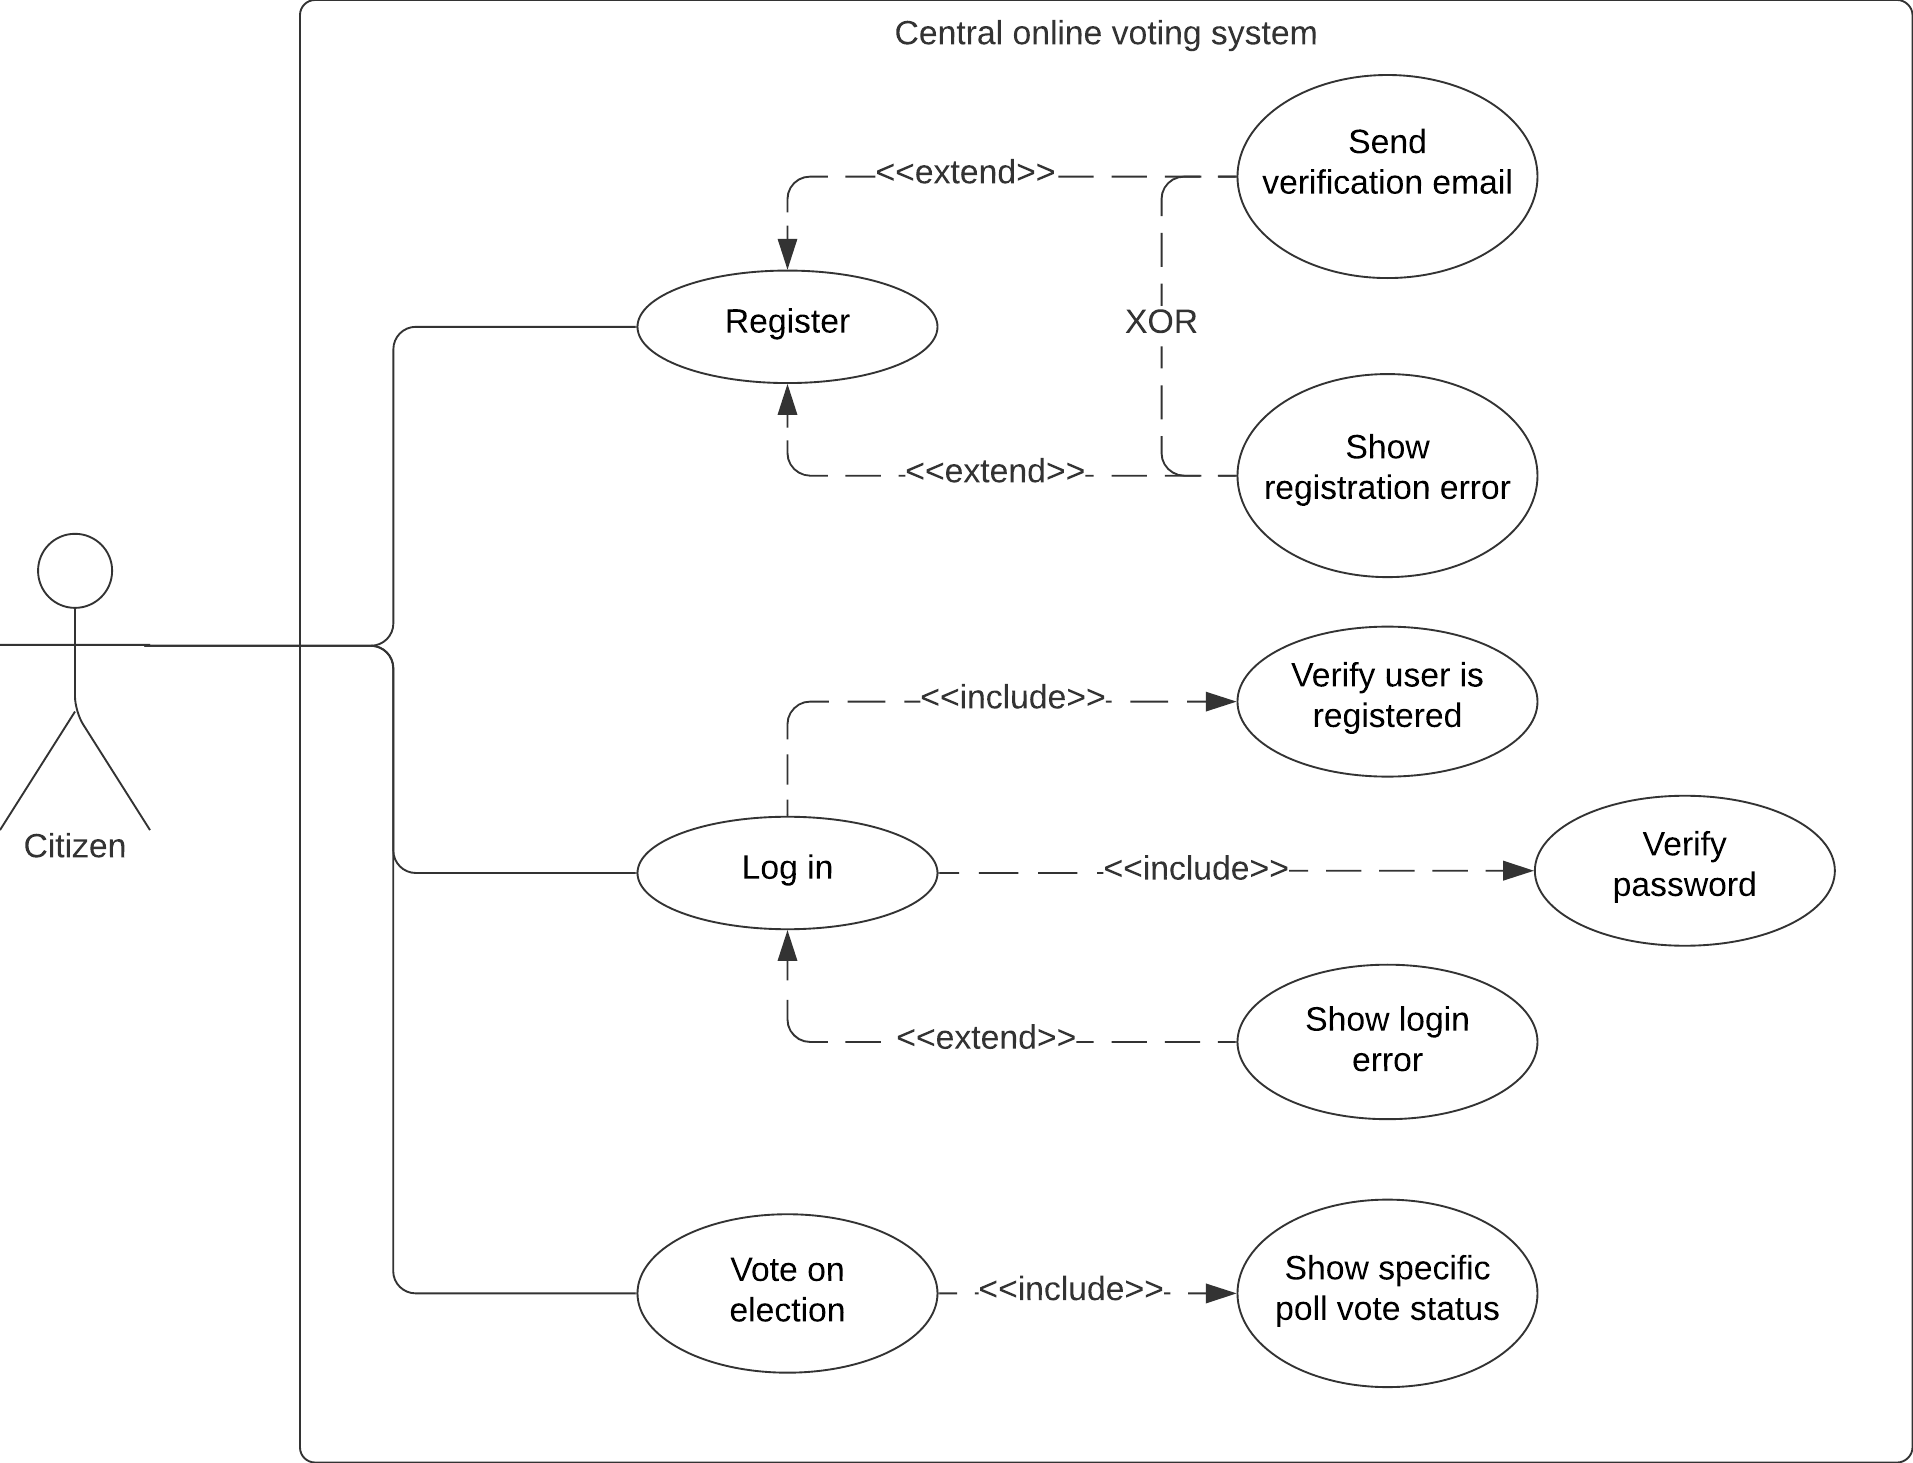
\includegraphics[width=\linewidth]{citizen_uml.png}
      \caption{Citizen use case UML for \Title}
      \label{fig:citizen_uml}
    \end{figure}

    Figure \ref{fig:citizen_uml} shows available use cases for citizen. He can register and in that case he will receive an email, 
    or he can see some error regarding registration. Citizen can try to login, which will trigger checks if he is registered and that password matches.
    In case of any errors, he will see a message. 
    Citizen can vote, and after that he will see status of his vote regarding every poll in the election, no matter if vote is valid or not.
    \pagebreak

    \subsection{Ward administrator use case UML}
    \begin{figure}[h]
      \centering
      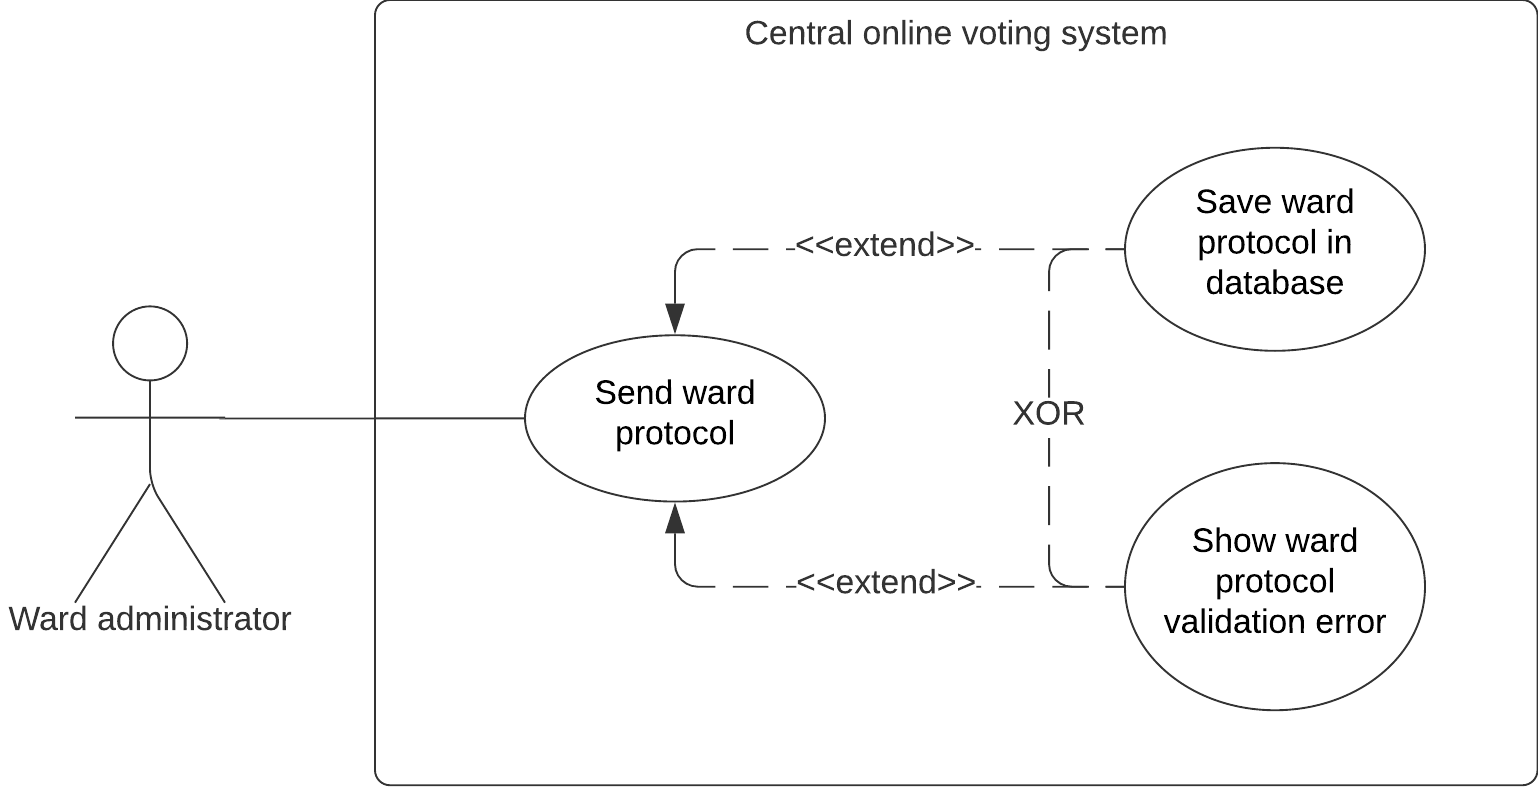
\includegraphics[width=0.65\linewidth]{ward_admin_uml.png}
      \caption{Ward administrator use case UML for \Title}
      \label{fig:ward_admin_uml}
    \end{figure}

    Figure \ref{fig:ward_admin_uml} shows available use cases for ward administrator. Ward administrator can try to send ward protocol.
    If anything is not correct in protocol he tried to send, he will see a validation error, and protocol will not be send.

    \subsection{Committee administrator use case UML}
    \begin{figure}[h]
      \centering
      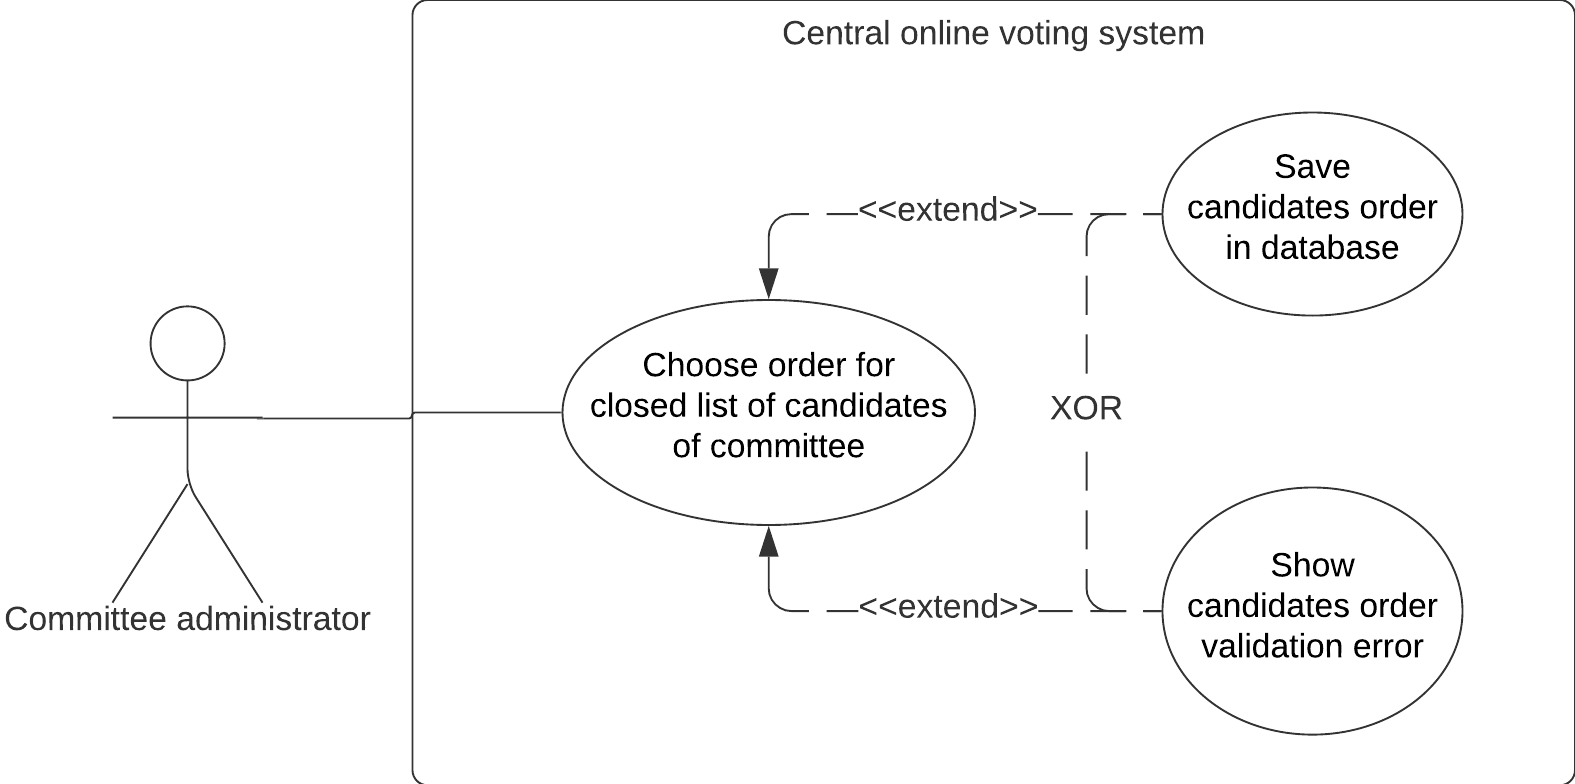
\includegraphics[width=0.65\linewidth]{committee_admin_uml.png}
      \caption{Committee administrator use case UML for \Title}
      \label{fig:committee_admin_uml}
    \end{figure}

    Figure \ref{fig:committee_admin_uml} shows available use cases for committee administrator. Committee administrator can try to send closed list candidates' order.
    If anything is not correct in the order of candidates, he will see a validation error, and candidates order will not be saved.
    \pagebreak

    \subsection{Administrator use case UML}
    \begin{figure}[h]
      \centering
      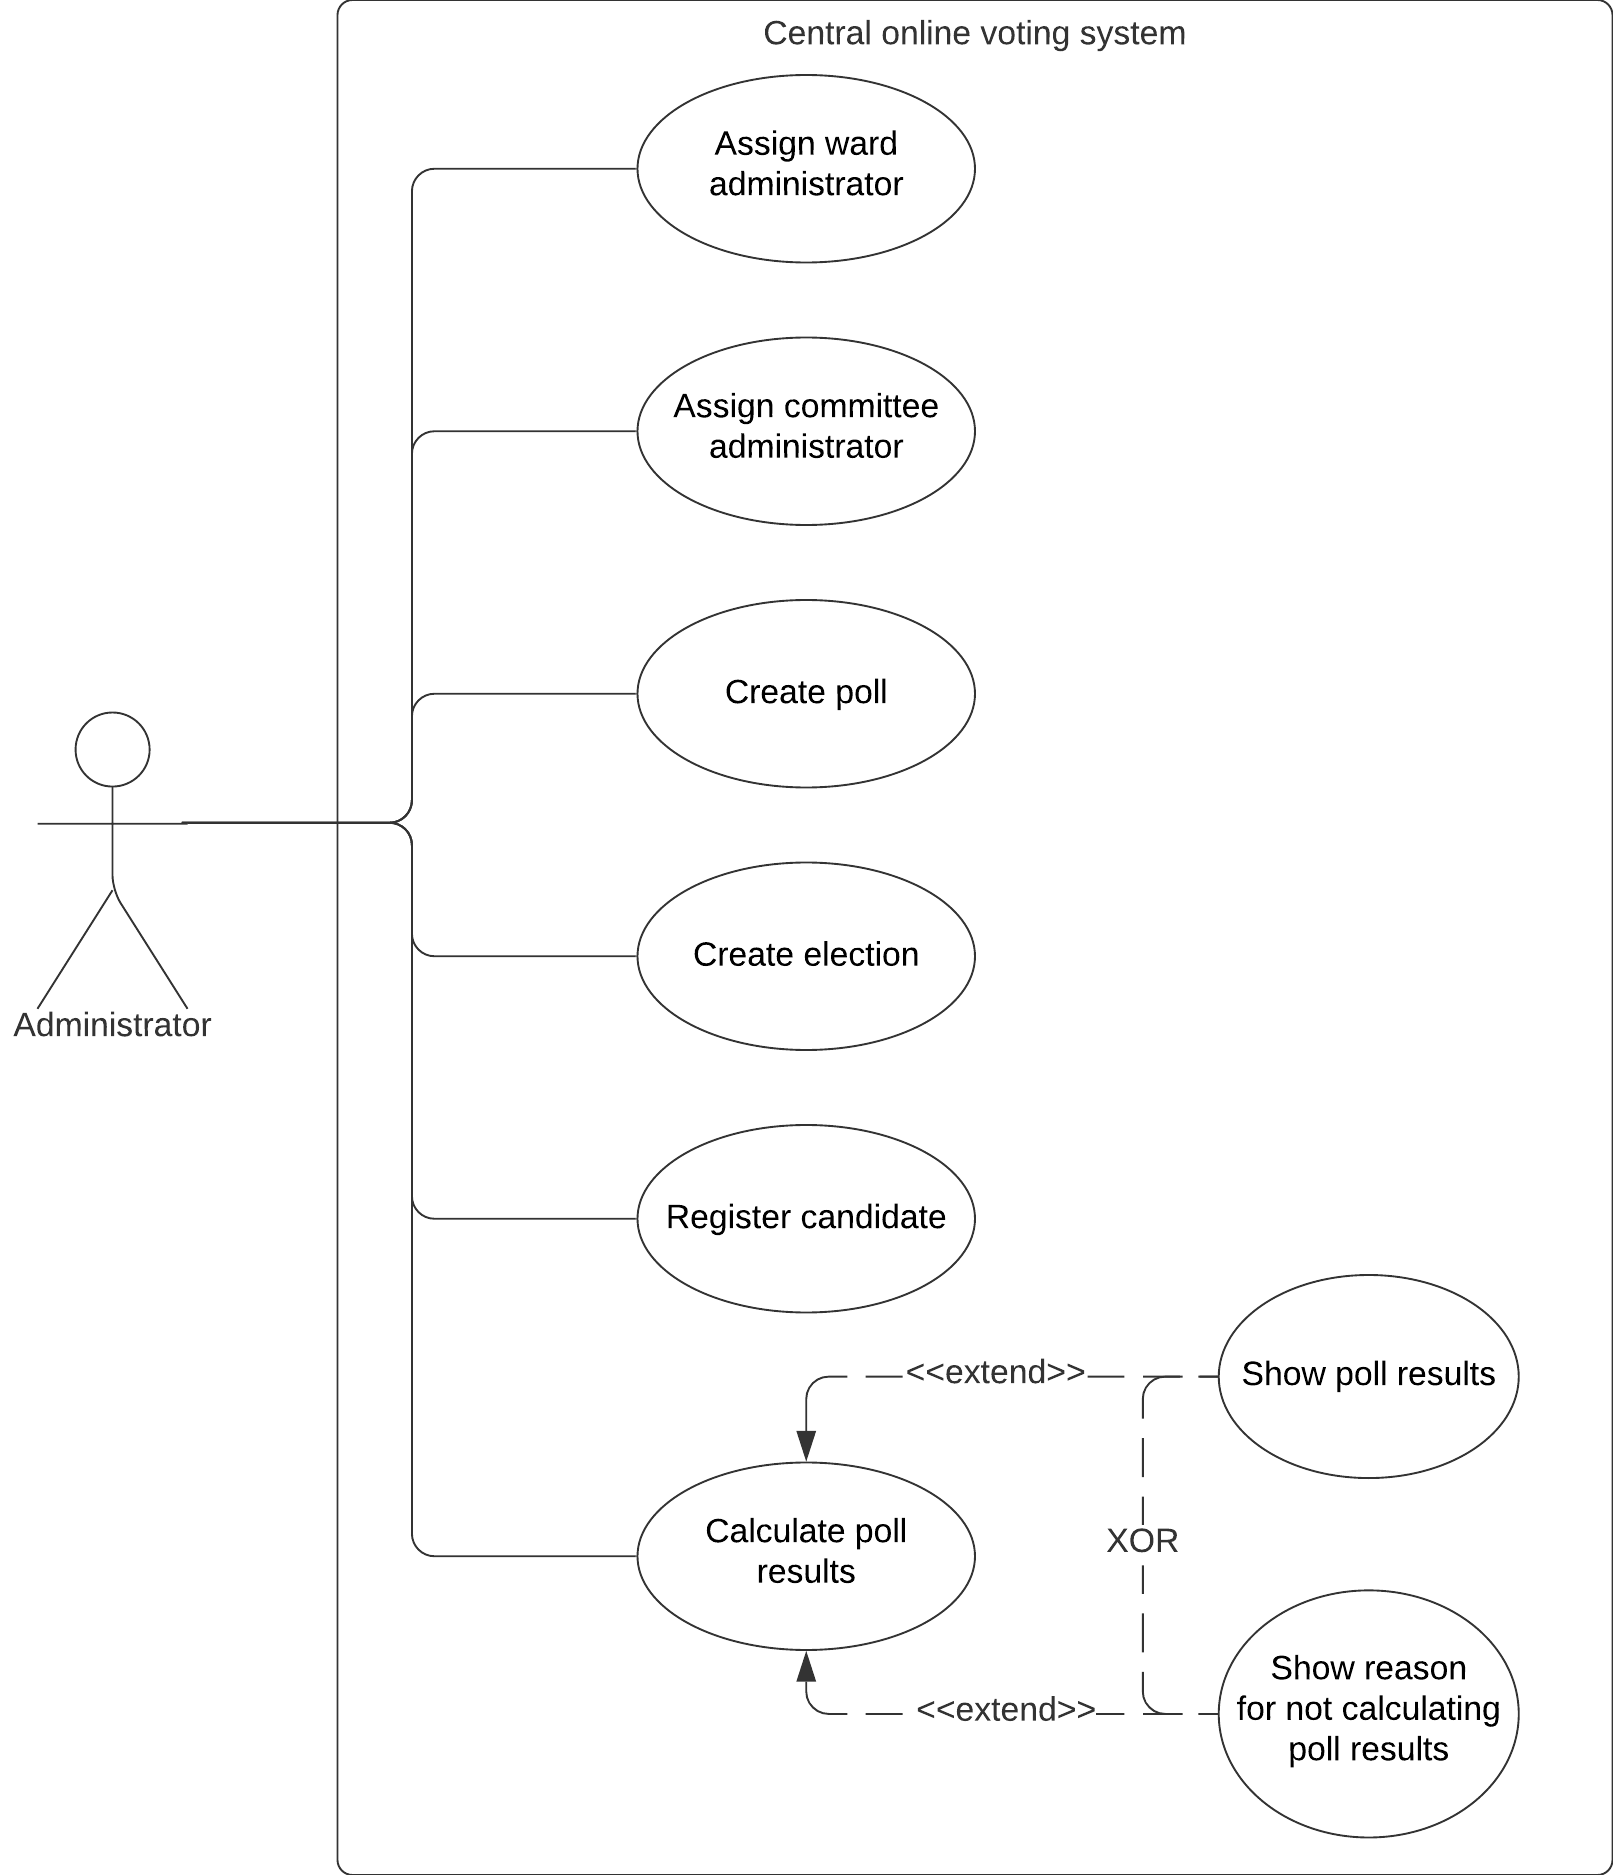
\includegraphics[width=0.8\linewidth]{admin_uml.png}
      \caption{Administrator use case UML for \Title}
      \label{fig:admin_uml}
    \end{figure}

    Figure \ref{fig:admin_uml} shows available use cases for administrator. We assume that administrator knows what he is doing, so there is no need to validate his choices.
    However, he has no power over how many protocols are sent from wards when he wants to calculate poll results. 
    Thus he will get appropriate message when he tries to calculate results of poll that is not ready to be calculated.

  \section{Description of tools}
    Application is developed in Java programming language, with use of Spring Framework and Thymeleaf as template engine. 
    Data is stored in MySQL database, and whole application is build with help of Apache Maven build automation tool.

    \subsection{Java}
      It's object--oriented programming language that requires Java Virtual Machine to run a program. 
      This allows Java applications to run on almost every device, regardless of it's operational system\cite{bib:horstmann2008core}.
      Java offers huge open--source ecosystem.

      \subsubsection{Alternative}
        C\# - It's also object--oriented programming language, but it's used to develop software for Microsoft platforms\cite{bib:thai2003net}.

      Although there is no much difference in beginner level development between Java and C\#, I find C\# less convenient than Java,
      because I use machine with macOS operating system as my everyday work tool, and Java has huge support on Unix based system, compared to almost none support for C\#.

    \subsection{Maven}
      Apache Maven is a tool that is capable of building and managing any Java-based project. 
      It helps developers with dependency management, as it's able to download all necessary dependencies with almost no participation of developer.
      It's easy for beginners, as it's build lifecycles and syntax is easy to understand---all You need is artifact info of dependency that You want to include in Your project, 
      and it will download and include dependency in project during install build lifecycle\cite{bib:maven}.

      \subsubsection{Alternatives}
        \paragraph{Gradle}
          It's also application build tool for Java-based projects. It's better than Maven for larger projects, thanks to better automation methods and better performance.
          Gradle is built with more experienced and demanding developer in mind\cite{bib:gradle}.
        
        \paragraph{Ant}
          Ant is a powerful tool that allows developer to automate very complicated task, but this functionality is not cheap.
          It's complicated to configure and it's being ousted by Gradle\cite{bib:ant}.

      \paragraph{} %I know it's probably not the way to achieve this result, but it works
      I chose Maven because I wanted to learn modern build technology that is common in the industry, but is suitable for beginners.

    \subsection{Spring}
      It's an open--source framework for Java platform. It focuses on delivering out--of--the--box core features for any kind of application, 
      so developers can focus on business logic of the application. 
      Aside from Spring Core, which provides easy dependency injection, Spring provides extensions in form of more or less independent modules, each available as it's own maven artifact.\cite{bib:spring}
      Spring Boot is an extension of Spring framework, which provides out--of--the--box configuration, and requires user to provide only application specific configuration.
      
      \subsubsection{Alternative}
        Because Spring is open--source framework, considered a standard in the industry for over 10 years, there is no other framework that is as feature--packed as Spring.
        One could make a case for .Net framework for C\# language, but it's developed and directed by Microsoft\cite{bib:thai2003net}, 
        whereas Spring is powered by community, and contains features required by that same community. 

      \subsubsection{Spring Security}
        Authentication and Authorization framework for Spring based applications. Provides quick protection of API exposed by application and
        integration with users in database. Allows for assigning users' roles, and managing accesses based on these roles\cite{bib:spring_security}.

      \subsubsection{Spring Web MVC}
        It's designed around front controller pattern, and helps developers follow the Model--View--Controller design pattern.
        It coordinates flow of request processing performed by configurable delegate components\cite{bib:spring_web_mvc}.
      
      \subsubsection{Spring Data JPA}
        Spring implementation of JPA contract, powered by Hibernate. Reduces hugely boilerplate code that's associated with querying database,
        especially with Repository interface custom finder methods\cite{bib:spring_data_jpa}.

    \subsection{Thymeleaf}
      Modern server-side Java template engine resolver. 
      It converts HTML files with Thymeleaf--specific dynamic attributes based on model attributes provided by developer through Spring MVC framework\cite{bib:thymeleaf}.
      
      \subsubsection{Alternative}
        There are not many pure alternatives when it comes to template resolvers. 
        Java Enterprise Edition comes with JSP, which is not pleasant to use, and is considered obsolete.
        It definitely does not provide level of integration with Spring MVC framework as much as Thymeleaf does.

  \section{Methodology of design and implementation}
    Base of every application is a well designed database schema. 
    Once schema is considered with required functionalities of application in mind, and with space for extensibility predicted,
    it makes development not only go faster and more efficient, but also more pleasant for developer.

    With proper database schema, we have to consider what is the best way for user to use our application---through web browser or application?
    Because application is meant to be nation--wide, 
    and there is a web browser on perhaps every computer with internet connection---which is necessary for application to work---web application is the way to go.
    
    When designing web application, we have to decide how we want to achieve end result---presenting view to application user.
    There are two most common approaches when it comes to Spring application:
    \begin{itemize}
      \item Exposing REST API from Spring application, that contains all of business logic and create another application, that consumes that API and interacts with the user in any way desired.
      \item Keep view rendering on server side, and expose pure html to the user.
    \end{itemize}
    I chose the second option, because it is not the most important thing for \Title to be pretty and responsive, I wanted to focus on backend side of the application.

    Once view presenting is established, we want to consider how we want to design architecture of the application.
    I can see two approaches in choosing the architecture: basing on application requirements or basing on technology used in application.
    Because Spring provides whole framework dedicated to MVC design pattern, and also it's widely used in the industry, I chose to develop application in that manner,
    rather than choosing architecture basing on application requirements. 
    My application is not large enough to be hugely impacted by bad architecture. I could only harm my project by using some fancy architecture.

\chapter{External specification}
  \section{Types of users}



\chapter{Internal specification}

\begin{itemize}
\item 
\end{itemize}



\chapter{Verification and validation}

\begin{itemize}
\item 
\end{itemize}

 
 
\chapter{Conclusions}

\begin{itemize}
\item 
\end{itemize}

 


%%%%%%%%%%%%%%%%%%%%%%%%%%%%%%%%%%%%%%%%%%
\backmatter
\pagenumbering{Roman}
\stepcounter{PagesWithoutNumbers}
\setcounter{page}{\value{PagesWithoutNumbers}}

\pagestyle{onlyPageNumbers}

%%%%%%%%%%% bibliography %%%%%%%%%%%%
\bibliographystyle{plain}
\bibliography{thesis}

%%%%%%%%%  appendices %%%%%%%%%%%%%%%%%%% 

\begin{appendices} 

\chapter*{List of abbreviations and symbols}

\begin{itemize}
  \item[API] Application Programming Interface
  \item[HTML] HyperText Markup Language
  \item[MVC] Model--View--Controller 
  \item[REST] Representational State Transfer
  \item[UML] Unified Modeling Language
  \item[JPA] Java Persistence API
  \item[JSP] JavaServer Pages
\end{itemize}


\chapter*{Listings}

\chapter*{Contents of attached CD}

The thesis is accompanied by a CD containing:
\begin{itemize}
\item thesis (\LaTeX\ source files and final \texttt{pdf} file),
\item source code of the application,
\item test data.
\end{itemize}
 

\listoffigures
\listoftables
	
\end{appendices}


\end{document}


%% Finis coronat opus.